\begin{frame}
  \frametitle{Memoria}
  \begin{itemize}
	  \item La organización y administración de la \textit{memoria RAM} es uno de los factores más importantes en el diseño de un SO
	  \item Los programas y datos deben residir en ella para:
	  \begin{itemize}
	  	\item Poder ejecutar
	  	\item Referenciarlos directamente
	  \end{itemize}
  \end{itemize}
\end{frame}

\begin{frame}
  \frametitle{Memoria (cont.)}
  \begin{itemize}
	  \item La parte del SO que administra esta memoria se llama ``\textit{administrador de la memoria}'':
	  \begin{itemize}
	  	\item Lleva un registro de las partes de la memoria que se están utilizando y de aquellas que no
	  	\item Asigna espacio en memoria a los procesos cuando estos la necesitan
	  	\item Libera espacio de momoria asignada a procesos que han terminado
	  \end{itemize}
	  \item Se espera que el SO haga uso eficiente de esta memoria con el fin de alojar el mayor número de procesos $\rightarrow$ repercute en la \emph{multiprogramación}
  \end{itemize}
\end{frame}

\begin{frame}
  \frametitle{Direccionamiento}
  \begin{itemize}
	  \item \textbf{Dirección Lógica}:
	  \begin{itemize}
	  	\item Es una dirección que enmascara o abstrae una dirección física
	  	\item Referencia a una localidad en memoria
	  	\item Se la debe traducir a una dirección física
	  \end{itemize}
	  \item \textbf{Dirección Física}:
	  \begin{itemize}
	  	\item Es la dirección real. Es con la que se accede efectivamente a memoria
	  	\item Representa la dirección absoluta en memoria principal
	  \end{itemize}
	  \item La CPU trabaja con direcciones lógicas. Para acceder a la memoria se deben transformar en direcciones físicas
	  \item El mapeo entre direcciones virtuales y físicas se realiza mediante \emph{hardware} $\rightarrow$ \textbf{MMU} (Memory Management Unit)
  \end{itemize}
\end{frame}

\begin{frame}
  \frametitle{Traduccion \textbf{MMU}}
  \begin{figure}
    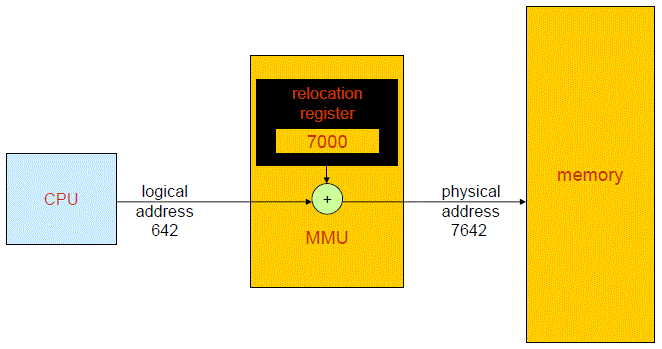
\includegraphics[scale=0.4]{images/mmu.png}
  \end{figure}
\end{frame}

\begin{frame}
  \frametitle{Asignación de memoria}
  \begin{itemize}
	  \item \textbf{Particiones Fijas}:
	  \begin{itemize}
	  	\item La memoria se divide en particiones o regiones de tamaño fijo $\rightarrow$ tamaños iguales o diferentes
	  	\item Alojan un proceso en cada una
	  	\item Cada proceso se coloca en alguna partición de acuerdo a algún criterio:
	  	\begin{itemize}
	  		\item \textbf{First Fit}
	  		\item \textbf{Best Fit}
	  		\item \textbf{Worst Fit}
	  		\item \textbf{Next Fit}
	  	\end{itemize}
	  \end{itemize}
	  \item \textbf{Particiones Dinámicas}:
	  \begin{itemize}
	  	\item Las particiones varían en tamaño y número
	  	\item Alojan un proceso cada una
	  	\item Cada partición se genera en forma dinámica del tamaño justo que necesita el proceso
	  \end{itemize}

	  \pause
	  \hspace{35pt} \textcolor{orange}{¿Qué problemas se generan en cada caso?}
  \end{itemize}
\end{frame}

\begin{frame}
  \frametitle{\textbf{Fragmentación}}
  \begin{itemize}
  	  \item La fragmentación se produce cuando una localidad de memoria no puede ser utilizada por no encontrarse en forma contigua
	  \item \textbf{Fragmentación Interna}:
	  \begin{itemize}
	  	\item Se produce en el esquema de particiones fijas, por ejemplo
	  	\item Es interna a la localidad asignada
	  	\item Es la porción de la localidad que queda sin utilizar
	  \end{itemize}
	  \item \textbf{Fragmentación Externa}:
	  \begin{itemize}
	  	\item Se produce en el esquema de particiones dinámicas, por ejemplo
	  	\item son huecos que van quedando en la memoria a medida que los procesos finalizan
	  	\item Al no encontrarse en forma contigua puede darse el caso de que tengamos memoria libre para alocar un proceso, pero que no la podamos utilizar
	  	\item Solución $\rightarrow$ \emph{compactación} $\rightarrow$ muy costosa
	  \end{itemize}
  \end{itemize}
\end{frame}

%%%%%%%%%%%%%%%%%%%%%%%%%%%%%%%%%%%%%%%%%%%%%%%%%%%%%%%%%%%%%%%%%%

\begin{comment}

\begin{frame}[fragile]
  \frametitle{Características - Configuración de discos (cont.)}
  \begin{itemize}
	  \item A futuro, todos los dispositivos llamados hdX serán denominados sdX $\leftarrow$ Introducido en Debian/Squeeze
	  \item Por estas y otras razones se adoptan 4 mecanismos nuevos para nomenclar\footnote{\url{http://wiki.debian.org/Part-UUID}}:
	  \begin{itemize}
	  	\item Nombres persistentes por \textbf{UUID} (\small{Universal Unique Identifier}):
	  	\begin{lstlisting}
$ ls –l /dev/disk/by-uuid/
2d781b26-0285-421a-b9d0-d4a0d3b55680 -> ../../sda1
31f8eb0d-612b-4805-835e-0e6d8b8c5591 -> ../../sda7
		\end{lstlisting}
		\item Utilizando \textbf{labels}
		\begin{lstlisting}
$ ls -l /dev/disk/by-label
data -> ../../sdb2
data2 -> ../../sda2
		\end{lstlisting}
	  \end{itemize}
  \end{itemize}
\end{frame}

\begin{frame}
  \frametitle{Herramientas para particionar}
  \begin{itemize}
	  \item El particionado de un disco se lo puede realizar mediante:
	  \begin{itemize}
	  	\item Software destructivo: \textit{fdisk}
	  	\item Software no destructivo: \textit{fips}, \textit{gparted}
		\begin{figure}
		    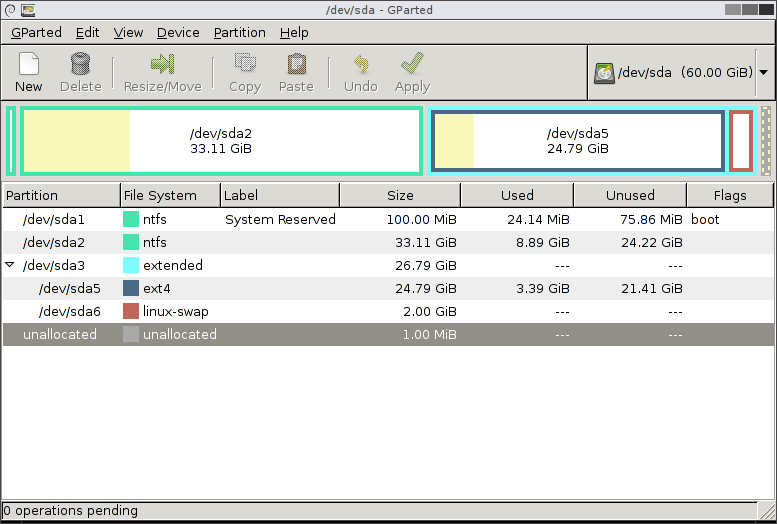
\includegraphics[scale=0.3]{images/gparted.png}
		\end{figure}
	  \end{itemize}
  \end{itemize}
\end{frame}

\begin{frame}[fragile]
  \frametitle{Permisos}
  \begin{itemize}
	  	\item Se aplican a directorios y archivos
	  	\item Existen 3 tipos de permisos y se basan en una notación octal:
	  	\begin{table}
		      \centering
		      \resizebox{10pc}{!}{
			  \begin{tabular}{| c | c | c |}
			      \hline
			      \bf Permiso & \bf Valor & \bf Octal \\
			      \hline
			      Lectura & R & 4 \\
			      \hline
			      Escritura & W & 2 \\
			      \hline
			      Ejecución & X & 1 \\
			      \hline
			  \end{tabular}
		      }
		\end{table}
		\item Se aplican sobre los usuarios:
		\begin{itemize}
			\item Usuario: permisos del dueño $\rightarrow$ \textbf{U}
			\item Usuario: permisos del grupo $\rightarrow$ \textbf{G}
			\item Usuario: permisos de otros usuario $\rightarrow$ \textbf{O}
		\end{itemize}
		\item Se utiliza el comando \textbf{chmod}:
		\begin{lstlisting}
$ chmod 755 /tmp/script
		\end{lstlisting}
  \end{itemize}
\end{frame}
\end{comment}